%-------------------------------------------------------------------------------
\section{Evaluation}
\label{sec:evaluation}
%-------------------------------------------------------------------------------

We evaluate our \Sys protocol implementation in an emulation study and answer
the following questions:
\vspace{-0.2cm}
\begin{enumerate}[noitemsep]
    \item What are the performance advantages of the \Sys protocol over the
     end-to-end, connection-splitting, and tunnel baselines in network settings
     with a lossy path segment near the data \textit{receiver}?
    \item How do the rateless and selective optimizations in \Cref
     {sec:eack:hints} impact the link overheads of the \Sys protocol?
    \item How much memory does the cache use at the proxy?
    \item How much traffic can a CPU-constrained proxy handle?
    % \item How do \Sys protocols perform in the real-world, and in the context of real Wi-Fi retransmissions?
\end{enumerate}

\subsection{Methodology}

\paragraph{Network configuration.}

We run emulation experiments in \texttt{mininet} to evaluate the \Sys protocol
in a controlled environment. We generally use a linear, two-segment network
topology.
The host nodes
correspond to the client, proxy, and server. Each segment has a bridging
node to emulate network properties on the link. In the multicast application,
we replicate the client and link it to the same bridging node.

We parameterize each path segment in three dimensions: delay, bandwidth, and a
random loss rate. We configure the network properties on the bridging nodes’
egress interfaces, using \texttt{tc-netem} to set delay and random loss,
and \texttt{tc-htb} to set bandwidth. Additionally, we use \texttt{tc-qdisc} to
configure the queues to use \texttt{red}, emulating congestive loss in our
single-flow environment. The links are symmetric.

In the end-to-end setting, the proxy simply runs a Linux transparent bridge.
Otherwise, the
proxy runs a binary for \Sys, the connection splitter, or the tunnel, that
manually bridges traffic between the two interfaces.
In the tunnel proxy case, we add an additional proxy
node near the client to transparently decapsulate traffic from the other
proxy.

\begin{table*}
    \centering
    \begin{tabular}{r l l l l l l}
        \toprule
        \bf
        & Data Receiver & Proxy $\leftrightarrow$ & eACK & Num & Cache & Reorder \\
        & (Client) $\leftrightarrow$ Proxy & Data Sender (Server) &  Frequency & Symbols & Capacity & Delay \\
        \midrule
         HTTP/3 & 2ms, 50 Mbit/s, 4\% loss & 30ms, 20 Mbit/s, 0\% loss & 10ms, 16pkts & 160+rateless & 48 kB & 30 ms \\
         Media & 50ms, 50 Mbit/s, 10\% loss & 100ms, 20 Mbit/s, 0\% loss & On NACK & 40+rateless & 20 kB & 110 ms \\
         Multicast & 10ms, 50 Mbit/s, 10\% loss & 30ms, 20 Mbit/s, 0\% loss & On NACK & 40+rateless & 64 kB & 30 ms \\
         \bottomrule
    \end{tabular}
    \caption{Experimental configuration of each  benchmark. The network settings
     represent scenarios with loss near the data receiver where the proxy is
     located behind a Wi-Fi access point, LEO satellite ground station, and
     cellular base station, respectively. The number of symbols is configured
     for the IBLT eACK, which in practice sends only a short prefix of symbols
     over the wire.
     % We also specify the quACK frequency,
     % cache capacity, and reorder delay in end-to-end signals.
     }
    \label{tab:experiment-config}
\end{table*}

\paragraph{Experimental configuration.}

\Cref{tab:experiment-config} describes the default experimental configuration
for each application. The network settings model scenarios with a lossy path
segment near the data receiver. The delay on the lossy link approximates the
location of the proxy relative to the data receiver---behind a Wi-Fi access
point, low-Earth orbit satellite ground station, or cellular base station.
The other link represents a reliable, but higher-delay path segment in the
network core. The bottleneck bandwidth is on this link, which
representing the congested backhaul. Importantly, the emulated loss is
attributed to non-congestive factors such as wireless interference.
% \thea{should there be something about choices of delays and BW?
% the intro to the low-latency media results presents delay as mimicking a
% satellite network - can you say something similar to that for all scenarios?}

% \Cref{tab:experiment-config} describes the default experimental configuration
%  for each application. The network settings model scenarios with a lossy path
%  segment located near the data receiver. We vary the delay on this lossy link
%  to approximate the location of an in-network proxy relative to the
%  receiver—for example, behind a Wi-Fi access point, a low-earth orbit satellite
%  ground station, or a cellular base station. The other link represents a
%  reliable but higher-delay segment in the cellular or wired network core, and
%  we model the backhaul as the bottleneck. Importantly, the emulated loss is
%  attributed to non-congestive factors such as wireless interference, rather
%  than queue overflows or network congestion.


The remaining configurations in \Cref{tab:experiment-config} are for the \Sys
protocol. We set the eACK frequency to the same as the protocol's underlying
acknowledgment scheme. The number of symbols determines how many missing
packets can be decoded between each eACK. Though the IBLT eACK needs more symbols
because of its non-determinism, choosing a large number of symbols minimally
impacts the encoding overhead, which scales logarithmically, and the link
overhead, because the sender can transmit only a prefix of symbols
with ratelessness.
The reorder delay is a client configuration that
must be at least the RTT to the proxy, which the client can learn from the \Sys
protocol. We also select a cache size that is small enough to evaluate
optimistic eviction in \Cref{sec:evaluation:memory}.

\paragraph{Measurement methodology.}

Unless otherwise specified, the HTTP benchmark results are the IQRs of
20 trials, and the media and multicast benchmark results are over 3 minutes.

We define spurious retransmissions as the number of packets sent by the server
containing duplicate frames. To measure link overheads, we record the values
of \texttt{/sys/class/net/<iface>/statistics/<metric>} for each emulated
network interface immediately before and after the benchmark. Cache memory
usage is measured by logging cache updates and parsing the time-series logs. We
use \texttt{rdtsc()} measure CPU cycles in the proxy.

% \Cref{tab:experiment-config} describes the parameters
% for each link to model---e.g., a lossy Wi-Fi or satellite path segment, or a reliable one in the core network with more congestion.

\paragraph{Hardware configuration.}

Experiments are performed on an AWS EC2 m4.xlarge instance with 16 GB of RAM
and 4-CPU Intel Xeon E5 processor at 2.30 GHz. The instance
runs Ubuntu 22.04.2 LTS with the Linux 6.80-1024-aws kernel.

\subsection{Main Results}

We find that
in-network retransmissions via the \Sys protocol enable a variety of performance
enhancements---higher throughput, lower latency, and lower link overheads than
end-to-end retransmissions---for a variety of encrypted transport protocols
when the data receiver is near a lossy path segment (\Cref{fig:perf}).
Our link-layer tunnels both harm and help performance depending on their
configurations, but they are transparent to the applications that share the link.
% The \Sys protocol enables similar improvements to connection-splitting PEPs without ossifying the protocol. Unlike link-layer retransmissions, the \Sys protocol can be tailored to each application.
% The \Sys proxy is on-path and doesn't fate share with the application nor incur encapsulation overheads, unlike transport-layer tunnels.

\paragraph{HTTP/3 file download.}
\Sys improves the throughput of a large HTTP/3 file download
$2.7\times$
% end-to-end 6.6720788246424245 at 4%
% packrat 18.30892838311422
% 18.3... / 6.67... = 2.744..
compared to end-to-end with 4\% loss on the near path segment (\Cref
{fig:perf:http}). End-to-end QUIC with CUBIC, in line with other studies on
``loss-based'' congestion control, achieves poor link utilization in even
minimally lossy environments. While the performance of CCAs differ by
implementation, \texttt{picoquic} CUBIC has been shown to be one of the more
aggressive ones~\cite{atc-submission}.

QUIC with a \Sys achieves similar throughput to QUIC with an explicit connection
splitter as loss increases. They both utilize nearly all available bandwidth
until $\approx\!10\%$ loss, before gradually deteriorating. In the split
connection, this behavior is due to the congestion window on the near path segment being
able to compensate for high loss with a short delay, to a certain threshold.
With \Sys, this is because the reorder delay initially hides loss from the congestion
control algorithm at the data sender. As the loss increases, we observe that the
proxy fails to decode the eACK more often and resets the connection. Each time
there is a reset, the receiver falls back to end-to-end retransmissions,
signaling more loss (and congestion) to the data sender.
This suggests that
the congestion response to loss with \Sys can be both as good and as fair as QUIC with a connection
splitter, without fate sharing or decrypting the connection at the proxy.

\begin{figure}[t]
    \centering
    \begin{subfigure}[b]{0.9\linewidth}
        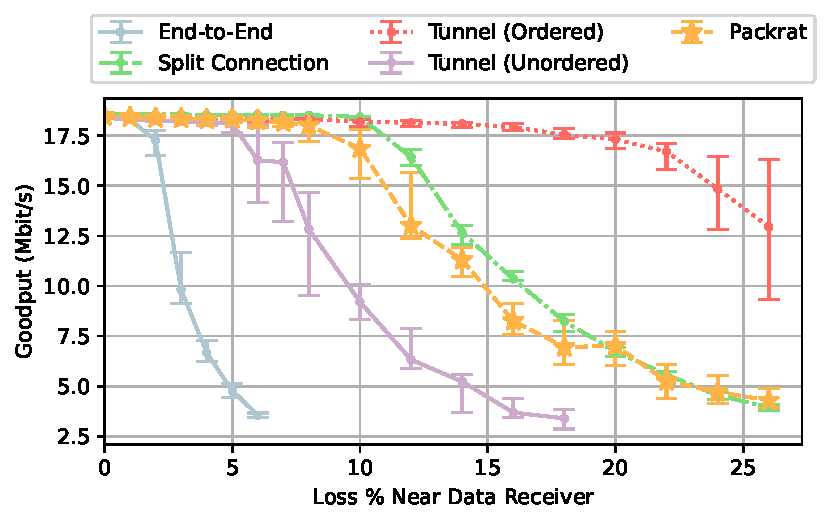
\includegraphics[width=\linewidth]{packrat-paper/figures/http_benchmark.pdf}
        \caption{QUIC HTTP/3 file download.}
        \label{fig:perf:http}
    \end{subfigure}
    \begin{subfigure}[b]{\linewidth}
        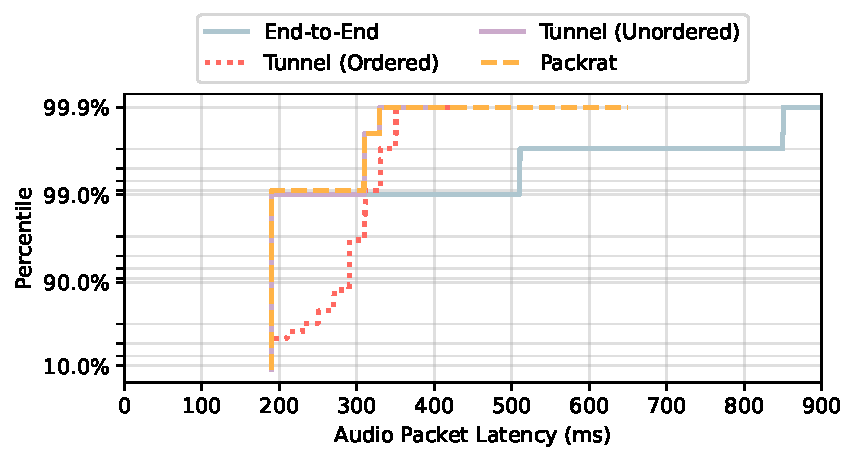
\includegraphics[width=\linewidth]{packrat-paper/figures/media_benchmark.pdf}
        \caption{Low-latency media stream with FEC.}
        \label{fig:perf:media}
    \end{subfigure}
    \begin{subfigure}[b]{\linewidth}
        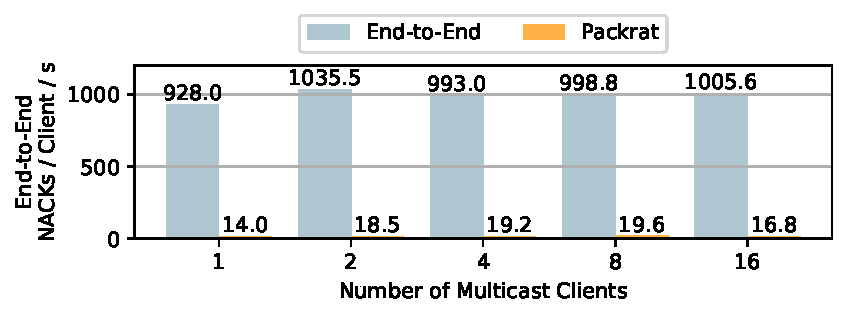
\includegraphics[width=\linewidth]{packrat-paper/figures/multicast_benchmark.pdf}
        \caption{Reliable IP multicast stream.}
        \label{fig:perf:multicast}
    \end{subfigure}
    \vspace{-0.3cm}
    \caption{The Packrat protocol achieves better throughput, latency, and link
     overheads in lossy network settings compared to end-to-end
     retransmissions. Applications using the tunnel differ in how much they
     benefit based on the tunnel configuration, which is a disadvantage of
     link-layer retransmissions.}
    \label{fig:perf}
\end{figure}

For the HTTP/3 download in this low-latency, low-loss
network setting, the ordered tunnel outperforms QUIC with a \Sys.
The unordered tunnel does not perform as
well because the retransmits at millisecond timesecales arrive out-of-order.
The end-to-end ACKs subsequently cause the server to send spurious
retransmissions (\Cref{fig:http:spurious}). The congestion response to spurious
retransmissions is not well-defined in standards, and \texttt{picoquic} makes some attempt
to revert the congestion window that leads to this result, which is a similar
result we observe when using \Sys with no reorder signal. The ordered tunnel does
not run into the same issues because its aggressive retransmissions, when
ordered, hide most loss the server could interpret as a congestion signal.
% \thea{Could you say something about how \Sys behaves when it comes to spurious retransmissions?
% This could be an opportunity to highlight why the ACK delays are impt.}
% Without modifying the end-to-end ACK signal, the data sender sends spurious retransmissions that the proxy has already retransmitted (\Cref{fig:http:spurious}). Note that these spurious retransmissions are of underlying QUIC frames, and the proxy would not be able to detect and withhold these since the sequence numbers are encrypted.
% The congestion response to spurious retransmissions is not well-defined, and a CCA implementation that receives the same end-to-end signals of loss will perform the same as end-to-end QUIC (\Cref{fig:http:fairness}). In other cases, the data sender may become confused about the consistent spurious retransmissions and perform strangely. Modified ACKs prevent this strange behavior.

\paragraph{Low-latency media with FEC.}

\Sys enables fewer and shorter stalls in a low-latency media stream over a
high-delay satellite network (\Cref{fig:perf:media}). In this network setting,
the minimum one-way latency of a packet is already 190 ms (40 ms encoding + 150 ms delay).
For reference, 150
ms is the normal latency for VoIP, and anything above produces a noticeable
drop in quality. Thus network-generated retransmissions are crucial in lossy, high-latency
settings.

Both \Sys and end-to-end benefit from FEC, but \Sys enables shorter stalls when
a frame still needs to be retransmitted. In this transport protocol, a frame
needs to be retransmitted if two packets are lost in a row. Thus at 10\% loss,
the 99th percentile delay of both mechanisms is the minimum of 190 ms. In the
remaining percentile, one more out-of-order packet arrives after $20$ ms,
draining the last of the buffer and generating an eACK or NACK. The length of
the stall is then the 100 or 300 ms RTT with the proxy or server. The unordered
tunnel exhibits a similar behavior to \Sys.
% to receive the retransmission and resume playback.

Unlike the HTTP/3 benchmark, this transport protocol gets none of the benefits
of FEC with the \textit{ordered} tunnel. When a retransmission is required, the
tunnel buffers at least 6 more packets until it receives the
retransmission and releases them to the client. The buffering
causes unnecessary stalls. If the tunnel had just released the
packets, a single missing packet would have been masked by the repetition
code.

\paragraph{Reliable IP multicast stream.}

Caching packets in the network like a CDN is inherently beneficial because it
can reduce the congestion in the core network. This is one of the idealistic
draws of IP multicast, but it is rarely used over the Internet in practice
because a reliable stream may require an overwhelming number of unicast
retransmissions from the server when there is loss. While CDNs and SFUs have
helped with content distribution, these are not options for encrypted transport
protocols without embedding trust in the network.

The \Sys proxy can handle in-network retransmissions for a large number of
multicast clients. Each client using the \Sys protocol sends on average $16.8$
end-to-end retransmissions/second, a $59\!\times$ reduction from $1005.6$
retransmissions/second/client without \Sys. This reduction scales with the
number of clients. In-network retransmissions reduce both the load at the
server and congestion in the network.\\

\noindent
The behaviors of the QUIC and media transport protocols with various tunnels
represent the challenges of configuring link-layer retransmissions
independently of the applications that share the link. A large download
over QUIC performs poorly
when there is excessive reordering, while the media transport protocol prefers
to receive packets right away.
Disabling link-layer retransmissions introduces loss, which can be even more
detrimental for performance.

\begin{figure*}[ht]
\centering
\begin{minipage}[t]{0.3\textwidth}
    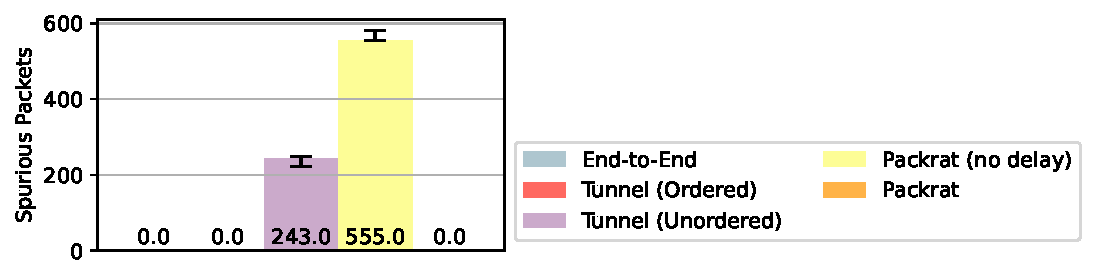
\includegraphics[width=\linewidth, trim=245 15 5 65, clip]{packrat-paper/figures/spurious_retx_legend.pdf}
    \begin{subfigure}[b]{\linewidth}
        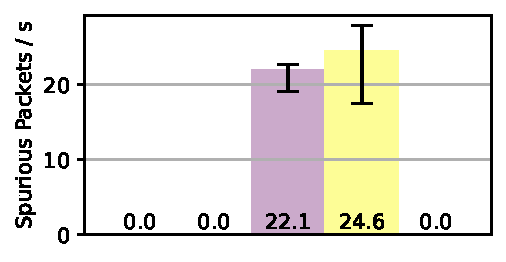
\includegraphics[width=\linewidth]{packrat-paper/figures/spurious_retx_http.pdf}
        \caption{HTTP/3 download.}
        \label{fig:http:spurious}
    \end{subfigure}
    \begin{subfigure}[b]{\linewidth}
        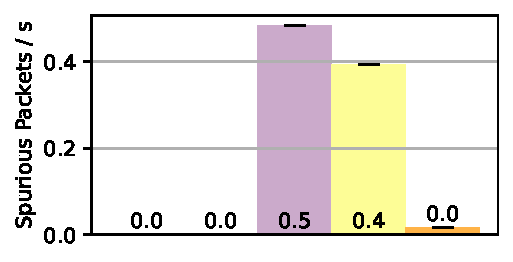
\includegraphics[width=\linewidth]{packrat-paper/figures/spurious_retx_media.pdf}
        \caption{Low-latency media.}
        \label{fig:media:spurious}
    \end{subfigure}
    \caption{The unordered tunnel and Packrat without modifying the end-to-end
     reorder signal cause the client to receive spurious retransmissions.
     Modifying the end-to-end signal with Packrat significantly reduces them.}
    \label{fig:spurious}
\end{minipage}%
\hfill
\begin{minipage}[t]{0.68\textwidth}
    \centering
    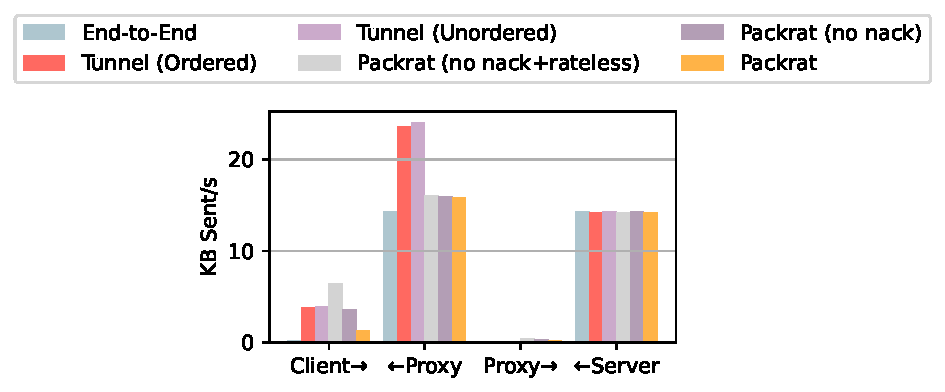
\includegraphics[width=0.9\linewidth, trim=5 140 5 5, clip]{packrat-paper/figures/network_stats_media_legend.pdf}
    % 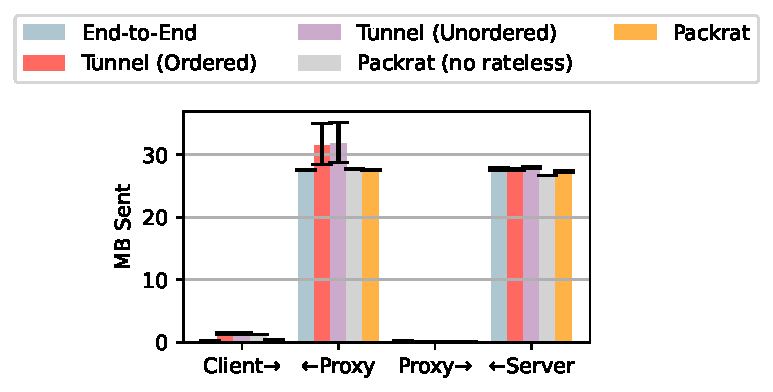
\includegraphics[width=0.7\linewidth, trim=5 140 5 5, clip]{packrat-paper/figures/network_stats_http_legend.pdf}
    
    \begin{subfigure}[b]{0.48\linewidth}
        \centering
        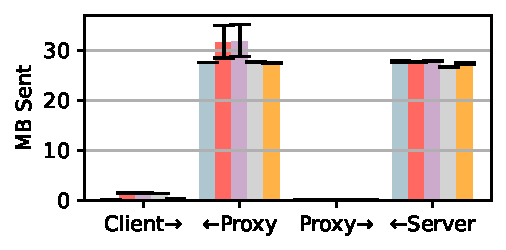
\includegraphics[width=\linewidth]{packrat-paper/figures/network_stats_http_tx_bytes.pdf}
        \caption{HTTP/3 download (bytes).}
        \label{fig:link-overheads:http-bytes}
    \end{subfigure}
    \begin{subfigure}[b]{0.51\linewidth}
        \centering
        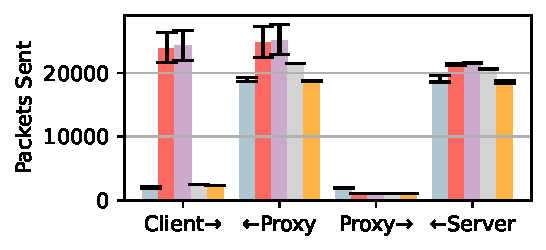
\includegraphics[width=\linewidth]{packrat-paper/figures/network_stats_http_tx_packets.pdf}
        \caption{HTTP/3 download (packets).}
        \label{fig:link-overheads:http-packets}
    \end{subfigure}\\

    \begin{subfigure}[b]{0.49\linewidth}
        \centering
        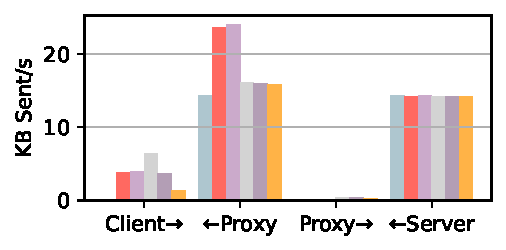
\includegraphics[width=\linewidth]{packrat-paper/figures/network_stats_media_tx_bytes.pdf}
        \caption{Low-latency media (bytes).}
        \label{fig:link-overheads:media-bytes}
    \end{subfigure}
    \begin{subfigure}[b]{0.49\linewidth}
        \centering
        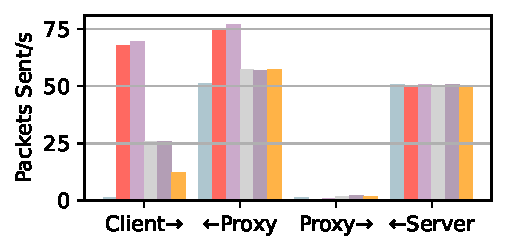
\includegraphics[width=\linewidth]{packrat-paper/figures/network_stats_media_tx_packets.pdf}
        \caption{Low-latency media (packets).}
        \label{fig:link-overheads:media-packets}
    \end{subfigure}
    
    \caption{The number of bytes (left) and packets (right) sent between the
     client, proxy, and server. The statistics are captured directly from the
     network interface. The link overheads from quACKs in the Packrat protocol are
     comparable to those of the underlying acknowledgment scheme. The client
     sends fewer bytes with rateless quACKs, and fewer packets when it
     selectively quACKs. The tunnel aggressively ACKs and retransmits.}
    \label{fig:link-overheads}
\end{minipage}
\end{figure*}

\subsection{Link Overheads}
\label{sec:evaluation:link-overheads}

% picoquic tx_bytes [198883.5, 27492622.0, 191807.5, 27736696.5]
% picoquic_rtunnel_retx7 tx_bytes [1435172.0, 31754825.0, 113619.0, 27963690.0]
% picoquic_rtunnel_retx7_ordered32 tx_bytes [1398215.0, 31516866.0, 103276.5, 27575304.5]
% picoquic_iblt_30ms tx_bytes [1266149.5, 27674317.0, 115277.0, 26672470.0]
% picoquic_iblt_30ms_hint tx_bytes [351208.0, 27494048.0, 110055.5, 27245627.0]

% picoquic tx_packets [2004.5, 18581.5, 1943.5, 18753.5]
% picoquic_rtunnel_retx7 tx_packets [24265.5, 25146.0, 1122.5, 21631.5]
% picoquic_rtunnel_retx7_ordered32 tx_packets [23867.0, 24750.0, 1026.5, 21327.0]
% picoquic_iblt_30ms tx_packets [2491.0, 21416.5, 1100.0, 20625.5]
% picoquic_iblt_30ms_hint tx_packets [2276.0, 18646.0, 1091.5, 18563.5]

% baseline tx_bytes [147.66572118181435, 14344.351371776342, 138.21977640181868, 14339.756587216456]
% baseline_rtunnel_retx7 tx_bytes [3925.3118199342766, 24075.523291814647, 108.52017350234354, 14317.224677303848]
% baseline_rtunnel_retx7_ordered32 tx_bytes [3834.258604701158, 23634.186568073015, 71.65183075616491, 14180.509943116185]
% iblt_delay110 tx_bytes [6397.578993802214, 16084.933839237683, 396.64150717354, 14215.75973782021]
% iblt_delay110_hint tx_bytes [3632.7542920194414, 15937.487922211047, 355.02262277865157, 14263.003369907003]
% iblt_delay110_hint_nack tx_bytes [1275.1961129433735, 15838.724627428588, 237.22743718841446, 14197.04110780209]

% baseline tx_packets [1.02550264090189, 50.93218798011756, 1.02550264090189, 50.87225600759732]
% baseline_rtunnel_retx7 tx_packets [69.38125902622755, 77.07585973692973, 0.8190704348042989, 50.7923556217056]
% baseline_rtunnel_retx7_ordered32 tx_packets [67.82618235752024, 75.36094504344966, 0.3129773276523932, 50.30278155502507]
% iblt_delay110 tx_packets [25.580860080034146, 57.12492729313365, 1.6248157905839729, 50.43255077863819]
% iblt_delay110_hint tx_packets [25.786554138093248, 57.040966852564985, 1.902104961153975, 50.60264656131202]
% iblt_delay110_hint_nack tx_packets [12.33599987063784, 57.105191303997195, 1.5582315626068852, 50.366172751184514]

% http packrat bytes volume = 351208.0 / ("" + 27245627.0) = 1.3%
% http end-to-end bytes volume = 198883.5 / (""+27736696.5) = 0.7%
% media packrat bytes volume = 1275.19611 / (""+14197.041107) = 8.2%
% media end-to-end bytes volume = 147.6657 / (""+14339.756) = 1.0%
In this section, we analyze how sending eACKs with the optimizations in \Cref
{sec:eack:hints} impacts the link overheads in the network.
\Cref{fig:link-overheads} displays the number of packets and bytes sent on each
link between the client, proxy, and server in the HTTP and media applications.
As a proportion of the volume in bytes sent by both endpoints of the
application, the HTTP client makes up $1.3\%$ of the traffic with \Sys and
$0.7\%$ without. The media client makes up $8.2\%$ of the traffic with \Sys
and $1.0\%$ without. We find that that we can reasonably think of eACKs as
control packets in the common case.
% , similar to TCP ACKs which are not congestion-controlled.


% http end-to-end tx_bytes 198883.5
% http packrat tx_bytes 351208.0
% http end-to-end tx_packets 2004.5
% http packrat tx_packets 2276.0
% media end-to-end tx_bytes 147.66572118181435
% media packrat tx_bytes 1275.1961129433735
% media end-to-end tx_packets 1.02550264090189
% media packrat tx_packets 12.33599987063784

\paragraph{Rateless eACKs.}
Using the rateless property to send smaller eACKs
% when the client can estimate how many retransmissions it expects
reduces the number of bytes the client sends by $3.6\!\times$ (\Cref
{fig:link-overheads:http-bytes}) and $1.8\!\times$ (\Cref
{fig:link-overheads:media-bytes}) compared to \Sys without the optimization.
% http sender tx_bytes 1266149.5 -> 351208.0
% 1266149.5/351208.0=3.6x
% media sender tx_bytes 6397.578993802214 -> 3632.7542920194414 -> 1.8x
This property allows clients to configure the number of symbols less
conservatively when initializing the \Sys connection while being able to
dynamically adjust to changing loss conditions, particularly in less controlled
non-emulation environments.

\paragraph{Sending eACKs on NACK.}

% media sender tx_packets 25.786554138093248 -> 12.33599987063784
Sending a eACK only when the client would otherwise send a NACK reduces the
number of packets the media client sends $1.9\!\times$ (\Cref
{fig:link-overheads:media-packets}). Note that without sending on NACK, we
configured the media client to eACK every other packet to balance latency with
frequent eACKing. The media client sends more packets than end-to-end because
although it only ACKs when there is a missing \textit{frame}, it eACKs when
there is a missing \textit{packet} because the FEC is opaque to the proxy.
% media sender tx_bytes 1275.1961129433735 -> 147.66572118181435
% 1127.53 * 8 = 9 Kbit

\paragraph{Base connection improvements.}

Even though the HTTP client eACKs at a similar frequency to which it ACKs, the
client sends a similar number of packets with and without the \Sys (\Cref
{fig:link-overheads:http-packets}). The proxy in the end-to-end scenario sends
nearly twice as many ACKs to the server because the number of ACKs depends on
the length of the connection. \Sys improves the throughput so much that the
number of net packets sent by the client are similar.

The IP multicast application demonstrates how \Sys can reduce congestion closer
to the server by caching retransmissions in the middle of the network (\Cref
{fig:perf:multicast}). This is especially impactful if the data is shared by
multiple clients.\\

\noindent Note that the tunnels aggressively ACK and retransmit in both
directions. The client sends $12$-$66\!\times$ additional packets compared to
end-to-end and the proxy sends $33$-$51$\% more to the client. Even though the
block ACKs are small, it can be costly for radios to switch often between
sending and receiving modes, and for proxies with per-packet overheads.

% media
% e2e 1.02550264090189, 50.93218798011756
% tunnel 69.38125902622755, 77.07585973692973
% ordered tunnel 67.82618235752024, 75.36094504344966
% receiver = 67.6 66.1x
% proxy = 1.51 1.48

% http 
% e2e 2004.5, 18581.5
% tunnel 24265.5, 25146.0
% ordered tunnel 23867.0, 24750.0
% receiver 12.1x 11.9x
% proxy 1.35x 1.33x


% \begin{figure}[t]
%     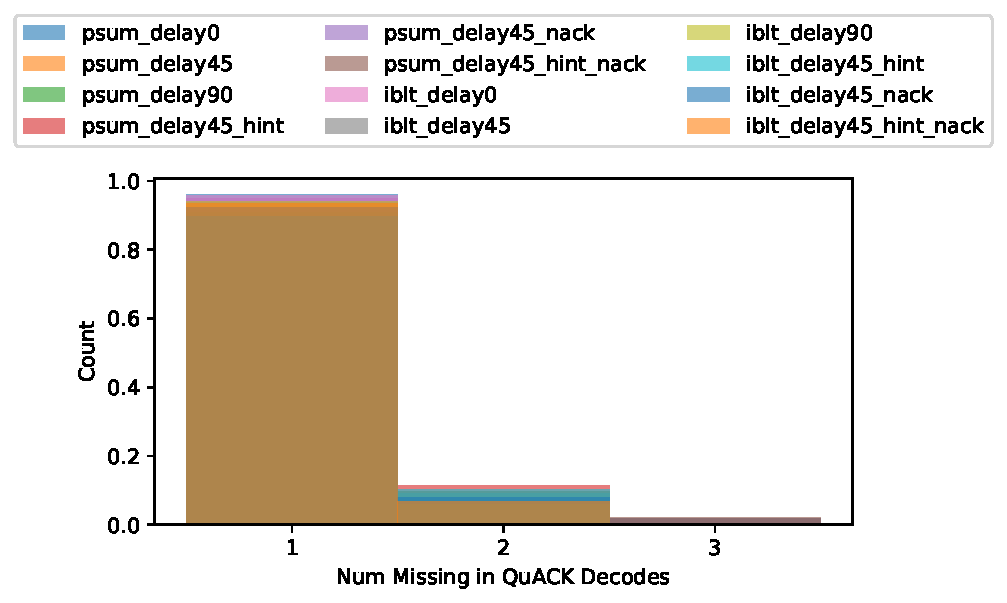
\includegraphics[width=\linewidth]{figures/decode_statistics.pdf}
%     \caption{Overlapping distributions of the number of missing packets decoded at the proxy for each application, for all eACKs received at a fixed threshold and frequency.}
%     \label{fig:quack-size-distribution}
% \end{figure}

\subsection{Memory Overheads}
\label{sec:evaluation:memory}

\begin{figure}[t]
    \centering
    \begin{subfigure}[b]{0.8\linewidth}
        \centering
        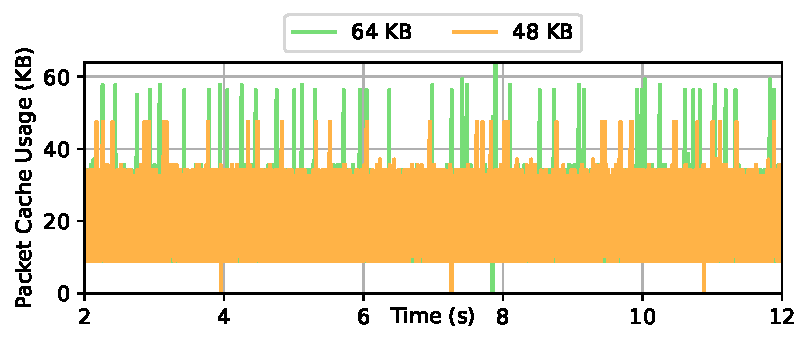
\includegraphics[width=\linewidth]{packrat-paper/figures/cache_http.pdf}
        \caption{HTTP/3 file download.
        % \thea{May be a non-issue, but not sure how to interpret the mass of orange here.}
        }
        \label{fig:memory:http}
    \end{subfigure}
    \begin{subfigure}[b]{0.8\linewidth}
        \centering
        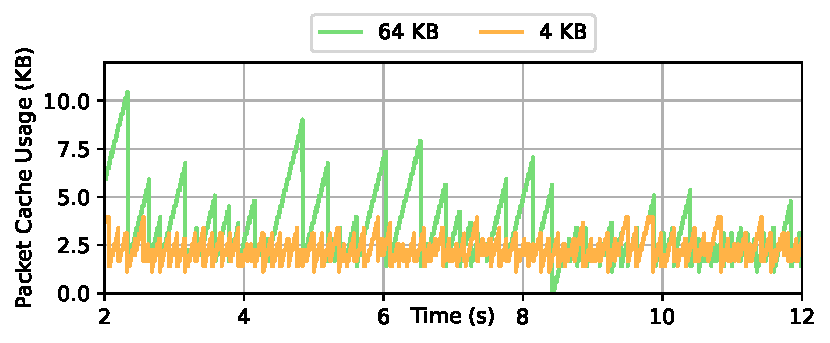
\includegraphics[width=\linewidth]{packrat-paper/figures/cache_media.pdf}
        \caption{Low-latency media with FEC.}
        \label{fig:memory:media}
    \end{subfigure}
    \caption{\small The number of bytes in the cache over a
     10-second period with both bounded (48 KB or 4 KB) and unbounded (64 KB)
     cache sizes. The proxy uses optimistic eviction if an incoming packet
     causes the cache to exceed its capacity.}
    \label{fig:memory}
\end{figure}

\begin{figure}[t]
    \centering
    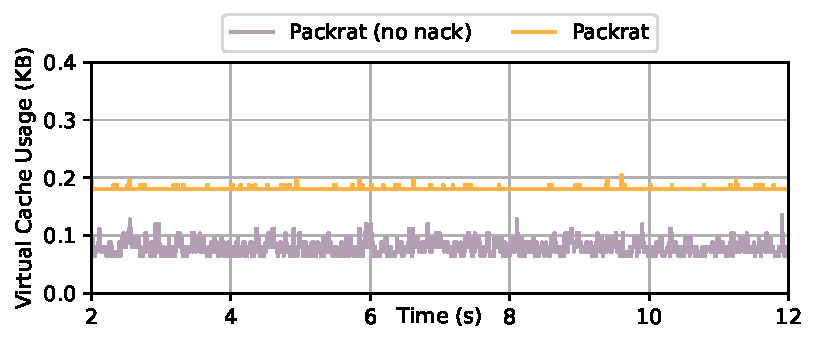
\includegraphics[width=0.8\linewidth]{packrat-paper/figures/cache_multicast.pdf}
    \caption{The sum of the virtual cache sizes of all $16$ clients in
     the multicast application. Each client uses $\approx\!$12 bytes each for a
     single insertion pair. The variations are due to individuals having
     slightly more or less than one insertion pair. Without selective quACKing
     (``no nack''), clients more often have empty virtual buffers. The base
     connection's packet cache (not pictured) is always 64 KB.}
    \label{fig:memory:multicast}
\end{figure}

We find that the \Sys proxy needs no more memory
than similar proxies for unencrypted transport protocols, and that the optimistic
eviction policy is an effective fallback for when the cache exceeds its memory limits.
Like any in-network retransmission mechanism,
the most significant memory usage at the proxy comes from the packet
cache. \Cref{fig:memory} shows the number of bytes in the packet contents of
the cache over a 10-second period of each application in our chosen
network settings. The maximum cache size
at the \Sys proxy is 64kB per connection, similar to a typical TCP window size.

% \thea{unclear to me what i should take away from this section.
% is it essentially just that these memory overheads are feasible and
% what we'd expect from any system that's buffering packets?
% could add a sentence at the beginning, end, and/or to each sub-section.}

\paragraph{HTTP/3 file download.}

The cache grows quickly because each data packet is large, but evicts
packets every 10~ms when
it receives an eACK (\Cref{fig:memory:http}). The minimum cache size is
$\approx\!10$ kB, the size of the outstanding packets between the client and
proxy. A spike occurs when an eACK is dropped, at which point the proxy
optimistically evicts. The proxy resets the connection if there is an
error, which is more common with a smaller cache, and drops the cache
size to 0.

\paragraph{Low-latency media with FEC.}

The media application relies on optimistic eviction to keep the cache small
since the client selectively eACKs (\Cref{fig:memory:media}). The
line plateaus at the maximum cache size because the proxy
assumes these packets have been received. The cache size only needs to fit 1-2
RTTs of packets between the client and proxy.

\paragraph{Reliable IP multicast stream.}

The multicast application has a fixed packet cache size of 64 kB, and we analyze
the memory overheads of the per-client virtual caches (\Cref
{fig:memory:multicast}). In particular, we calculate the overhead of each
virtual cache as 4 bytes for the first global index and then 8 bytes for each
insertion pair (\Cref{sec:implementation:proxy}). When there are 16 clients,
the proxy uses on average 0.178 KB in the virtual caches for a very low
overhead of 12 bytes/client. That is exactly one insertion pair, and in general
the overheads of the virtual caches are proportional to the number of
outstanding retransmissions.
% average = 0.17788111888111888 KB = 1

\subsection{CPU Overheads}

% \begin{table}[h]
%   \centering
  
%   \begin{subfigure}[b]{\linewidth}
%     \centering
%     \small
%     \begin{tabular}{ l l l l l }
%       \toprule
%         & \multicolumn{2}{l}{\bf Power Sum} & \multicolumn{2}{l}{\bf IBLT} \\
%         & Cycles & \% & Cycles & \% \\
%         \midrule
%         Sniff Packet & 100 & 100 & 100 & 100 \\
%         Table Lookup & 100 & 100 & 100 & 100 \\
%         Parse ID & 100 & 100 & 100 & 100 \\
%         Encode ID & 100 & 100 & 100 & 100 \\
%         Cache Add & 100 & 100 & 100 & 100 \\
%         Other & 100 & 100 & 100 & 100 \\
%         \midrule
%         \emph{Total} & \emph{22974} & \emph{100.0} & \emph{22975} & \emph{100.0} \\
%     \bottomrule
%     \end{tabular}
%     \caption{Data packets.}
%     \label{tab:cpu-overheads:data-packets}
%   \end{subfigure}
  
%   \begin{subfigure}[b]{\linewidth}
%   \centering
%   \small
%     \begin{tabular}{ l l l l l }
%       \toprule
%         & \multicolumn{2}{l}{\bf Power Sum} & \multicolumn{2}{l}{\bf IBLT} \\
%         & Cycles & \% & Cycles & \% \\
%         \midrule
%         Sniff Packet & 100 & 100 & 100 & 100 \\
%         Table Lookups & 100 & 100 & 100 & 100 \\
%         Deserialize & 100 & 100 & 100 & 100 \\
%         Decode QuACK & 100 & 100 & 100 & 100 \\
%         Cache Evict/Reorder & 100 & 100 & 100 & 100 \\
%         Retransmit (Optional) & 100 & 100 & 100 & 100 \\
%         Other & 100 & 100 & 100 & 100 \\
%         \midrule
%         \emph{Total} & \emph{22974} & \emph{100.0} & \emph{22975} & \emph{100.0} \\
%     \bottomrule
%     \end{tabular}
%     \caption{QuACKs.}
%     \label{tab:cpu-overheads:quacks}
%   \end{subfigure}
  
%   \caption{The breakdown of CPU cycles for the processing of each packet. Data packets may have large payloads that must be read entirely into user space to add to the packet cache. Both types of packets must update the cache either by inserting new packets or evicting and/or reordering existing packets. QuACKs typically have more complicated cache operations in addition to possible retransmits.}
%   \label{tab:cpu-overheads}
% \end{table}

% While it may be relatively inexpensive to encode and decode an eACK (\Cref
% {sec:eack:microbenchmarks}), identifying the missing packet identifiers is
% just one small part of the packet loop. Where else in packet processing does
% the proxy spend valuable CPU cycles?

% \paragraph{Data packet cycles.}

% The case of data packets is similar to when the sidekick connection is near the
% data \textit{sender} in that they both parse and encode the packet identifier,
% but differ in that the packet contents need to be added to the cache in case
% the packet later needs to be retransmitted (\Cref
% {tab:cpu-overheads:data-packets}). In our implementation, this requires reading
% additional bytes into memory compared to only reading sufficient bytes to parse
% the identifier, though this could potentially be alleviated by kernel bypass or
% zero-copy serialization techniques~\cite
% {dpdk,wan2022retina,raghavan2023cornflakes}. Additional cycles are also
% required to update the cache by inserting the packet.

% \paragraph{QuACK packet cycles.}

% Importantly, when the sidekick connection is near the data \textit
% {receiver}, the proxy must also handle incoming eACKs (\Cref
% {tab:cpu-overheads:quacks}). Outside of the orthogonal overheads of sniffing
% the packet, the eACK and cache operations are comparatively more expensive
% than for data packets. We use a ring buffer for the cache to make these
% operations as efficient as possible. Something comparing the total number of
% cycles to process each type of packet, but also the frequency of each of these
% packets relative to each other.

% \begin{table}[h]
%   \centering
% \begin{tabular}{ l l l }
%   \toprule
%     \textbf{Category} & \textbf{200 bytes} & \textbf{1500 bytes} \\
%     \midrule
%     No Proxy & 100 Mbit/s & 100 Mbit/s \\
%     Bridge & 100 Mbit/s & 100 Mbit/s \\
%     Sidekick & 100 Mbit/s & 100 Mbit/s \\
% \bottomrule
% \end{tabular}
%   \caption{\label{tab:proxy-throughput} Throughput of packets in the on-path proxy.}
% \end{table}

% \paragraph{Impact on available bandwidth.}

% We quantify the estimated impact of sidekick connections on the overall
% available bandwidth through the proxy in \Cref{tab:proxy-throughput}. We scale
% the load through the proxy by generating MTU-sized data packets at a fixed
% bandwidth, and generating eACKs in the reverse direction at the same frequency
% of \texttt{picoquic} ACKs, which is the more frequent of every 8 packets or 25
% ms. The sidekick proxy achieves XX\% lower throughput than the bridge proxy,
% which simply forwards packets. The difference between the bridge proxy and no
% proxy at all is not fundamental to the Sidekick protocol but any on-path
% proxy.

% We discuss some caveats for thinking about proxy CPU overheads.
% We note that this number assumes that \textit{all} connections going through the
% proxy receive sidekick assistance, when a subset is the more realistic
% scenario. It also assumes consistent loss, and a positive acknowledgment
% scheme. In contrast, a NACK scheme may generate smaller and less frequent
% eACKs, and loss in a real network scenario would also likely be more bursty
% and it would be more realistic to consider worst and average case performance.
% Finally, the overall throughput depends on the size of the data packets, as the
% data packet path depends on the size of the packet that is being read to the
% cache whereas the eACK frequency depends more on the overall number of
% packets.

In this experiment, we analyze the number of cycles that the proxy
needs to process each
packet in the HTTP/3 benchmark, and use the per-packet overheads to
extrapolate the capacity of a CPU-constrained proxy. These overheads
include both eACK operations and transport-protocol logic for e.g.,
packet triaging, loss detection, and cache management.

Each data packet on the base connection takes on average $1002$ cycles/packet.
The main overhead comes from adding the packet to a ring buffer used as the
packet cache.

Each eACK on the \Sys connection takes on average 27716 cycles/packet. The
proxy determines which packets to retransmit based on the eACK and evicts
packets. Loss detection involves encoding a delta of packets since the last
eACK into the existing state, as well as decoding the received eACK. Encoding
uses a total of $7156/27716 = 25.8\%$ of the cycles and decoding $3560/27716 =
12.8\%$. With a total of $38.6\%$ of the processing time spent on IBLT
operations, this implies that encoding and decoding are valuable to optimize.
% \thea{Are these results for both IBLT and psum?}

% psum
% WARN [proxy::cycles] transport
% WARN [proxy::cycles] 953 (total=101000,prop=1.000)
% WARN [proxy::cycles] transport,encode,decode
% WARN [proxy::cycles] 32923,9572,2984 (total=6800,prop=1.000,1.000,0.789)

% iblt
% WARN [proxy::cycles] transport
% WARN [proxy::cycles] 1002 (total=101000,prop=1.000)
% WARN [proxy::cycles] transport,encode,decode
% WARN [proxy::cycles] 27716,7156,3560 (total=6200,prop=1.000,1.000,0.516)

In this application, there is approximately one eACK for every $16.3$ data
packets. If each data packet uses a full MTU of 1500 bytes, this means a single
core of a 2.4 GHz CPU on a proxy would theoretically be able to handle 10.7
Gbit/s\footnote{ $2.4\text{ Gcycles/s }
\times(16.3 \text{ data packets } / (27716\cdot1 + 1002\cdot16.3) \text{ cycles })
\times (1500 \text{ bytes/data packet })
\times (8 \text{ bits/byte })
= 10.7 \text{ Gbit/s}$.
}. However, this estimate does not account for the substantial CPU overhead
involved in reading and writing to the NIC---these can be significantly reduced
using kernel bypass frameworks like DPDK or with specialized networking
hardware.

% iblt
% 2.4 Gcycles/s 
% * 16.29 data packets / (27716*1 + 1002*16.29) cycles
% * 1500 bytes / data packet
% * 8 bits / 1 byte
% = 10.7 Gbit/s.

% psum
% 2.4 Gcycles/s
% * 14.85 data packets / (32923*1 + 953*14.85) cycles
% * 1500 bytes / data packet
% * 8 bits / 1 byte
% = 11.2 Gbit/s

% \subsection{Raspberry Pi Experiments}

\subsection{Raspberry Pi Experiments}

\subsection{Raspberry Pi Experiments}

\input{figures_tex/real_world}

\Cref{fig:real-world} shows that \Sys protocols are robust in a real-world
environment even in the direction when the \Sys connection is near the
data \textit{receiver}. In the HTTP download application, \Sys increases the
long-lived throughput of the file download from XX MBit/s to XX Mbit/s---a
XX\% improvement. In the media application, \Sys reduces the 99th percentile
de-jitter latency XX\%, from XX to XX ms.

When thinking about real world scenarios that might benefit from \Sys, in this
case those with lossy path segments, one might reason that loss has all but
been eliminated in cellular and Wi-Fi networks by link-layer retransmissions.
However, \Cref{fig:real-world} demonstrates that there are tradeoffs with
configuring hardware retransmits, particularly in the media application.

In low-latency transport protocols such as media transfers, it can often be
desirable to drop frames instead of waiting for their retransmission as a
tradeoff between playback delay and smoothness. As we increase the number of
Wi-Fi retransmissions in the access point, the media application
actually...does something undesirable. In general, since link-layer
retransmissions are unilaterally applied to all connections that cross that
network path segment, it takes control out of co-existing applications to
determine the reliability guarantees that apply to them most.


\Cref{fig:real-world} shows that \Sys protocols are robust in a real-world
environment even in the direction when the \Sys connection is near the
data \textit{receiver}. In the HTTP download application, \Sys increases the
long-lived throughput of the file download from XX MBit/s to XX Mbit/s---a
XX\% improvement. In the media application, \Sys reduces the 99th percentile
de-jitter latency XX\%, from XX to XX ms.

When thinking about real world scenarios that might benefit from \Sys, in this
case those with lossy path segments, one might reason that loss has all but
been eliminated in cellular and Wi-Fi networks by link-layer retransmissions.
However, \Cref{fig:real-world} demonstrates that there are tradeoffs with
configuring hardware retransmits, particularly in the media application.

In low-latency transport protocols such as media transfers, it can often be
desirable to drop frames instead of waiting for their retransmission as a
tradeoff between playback delay and smoothness. As we increase the number of
Wi-Fi retransmissions in the access point, the media application
actually...does something undesirable. In general, since link-layer
retransmissions are unilaterally applied to all connections that cross that
network path segment, it takes control out of co-existing applications to
determine the reliability guarantees that apply to them most.


\Cref{fig:real-world} shows that \Sys protocols are robust in a real-world
environment even in the direction when the \Sys connection is near the
data \textit{receiver}. In the HTTP download application, \Sys increases the
long-lived throughput of the file download from XX MBit/s to XX Mbit/s---a
XX\% improvement. In the media application, \Sys reduces the 99th percentile
de-jitter latency XX\%, from XX to XX ms.

When thinking about real world scenarios that might benefit from \Sys, in this
case those with lossy path segments, one might reason that loss has all but
been eliminated in cellular and Wi-Fi networks by link-layer retransmissions.
However, \Cref{fig:real-world} demonstrates that there are tradeoffs with
configuring hardware retransmits, particularly in the media application.

In low-latency transport protocols such as media transfers, it can often be
desirable to drop frames instead of waiting for their retransmission as a
tradeoff between playback delay and smoothness. As we increase the number of
Wi-Fi retransmissions in the access point, the media application
actually...does something undesirable. In general, since link-layer
retransmissions are unilaterally applied to all connections that cross that
network path segment, it takes control out of co-existing applications to
determine the reliability guarantees that apply to them most.

